\documentclass[12pt]{article}

\usepackage{fullpage}
\usepackage{multicol,multirow}
\usepackage{tabularx}
\usepackage{listings}
\usepackage[utf8]{inputenc}
\usepackage[russian]{babel}
\usepackage{graphicx}
\usepackage{csquotes}

\begin{document}

\begin{titlepage}

    \begin{center}

        \bfseries
        {\small Московский авиационный институт\\ 
        (национальный исследовательский университет)}

        % \vspace{48pt}
        {\small Факультет информационных технологий и прикладной 
        математики}
        
        % \vspace{36pt}
        {\small Кафедра вычислительной математики и программирования}
        
        \vspace{8cm}
        {\Large Лабораторная работа \textnumero 5 по курсу} 
        \enquote{\Large Компьютерная графика}
        
    \end{center}
    
    \vspace{84pt}
    \begin{flushright}
        \begin{tabular}{rl}
            Студент: & Е.Ю. Юрков \\
            % Преподаватель: &  \\
            Группа: & М80-312Б-22 \\
            Дата: & \\
            Оценка: & \\
            Подпись: & \\
        \end{tabular}
    \end{flushright}
    
    \vfill
    
    \begin{center}
        
        \bfseries
        Москва, \the\year
    
    \end{center}

\end{titlepage}

% Выполнил студент группы М8О-312Б-22 МАИ \textit{Юрков Евгений}.

\subsection*{Цель лабораторной работы}

В этой лабораторной работе вы научитесь работать с техникой трассировки лучей для
создания реалистичной 3D-графики. Вы реализуете алгоритм Ray Tracing, который позволяет
рассчитывать физически корректные отражения, преломления, тени и свет в сцене.
Лабораторная работа подводит к пониманию основ рендеринга, работающего с лучами
света, а также к созданию реалистичных сцен.

\subsection*{Задача}

\textbf{Вариант 7. Отражения и текстурированные поверхности}

Постройте сцену с двумя текстурированными плоскостями (стена и пол) и одной сферой.
Реализуйте трассировку лучей с поддержкой текстурирования объектов.
Включите отражения на сфере и учтите отраженные текстуры на её поверхности.
Дополнительно: Реализуйте управление зеркальностью поверхности сферы для
изменения интенсивности отражений.

% \newpage
\subsection*{Метод решения}

Программа реализует сцену с использованием алгоритма трассировки лучей. Были реализованы классы фигур:
Plane и Sphere, каждый из которых имеет метод has\_hit, который вычисляет пересечение луча и фигуры,
причём класс плоскости вычисляет позицию пересечения, чтобы подставить цвет текстуры, соответствующий этой позиции.

\subsection*{Результат работы программы}

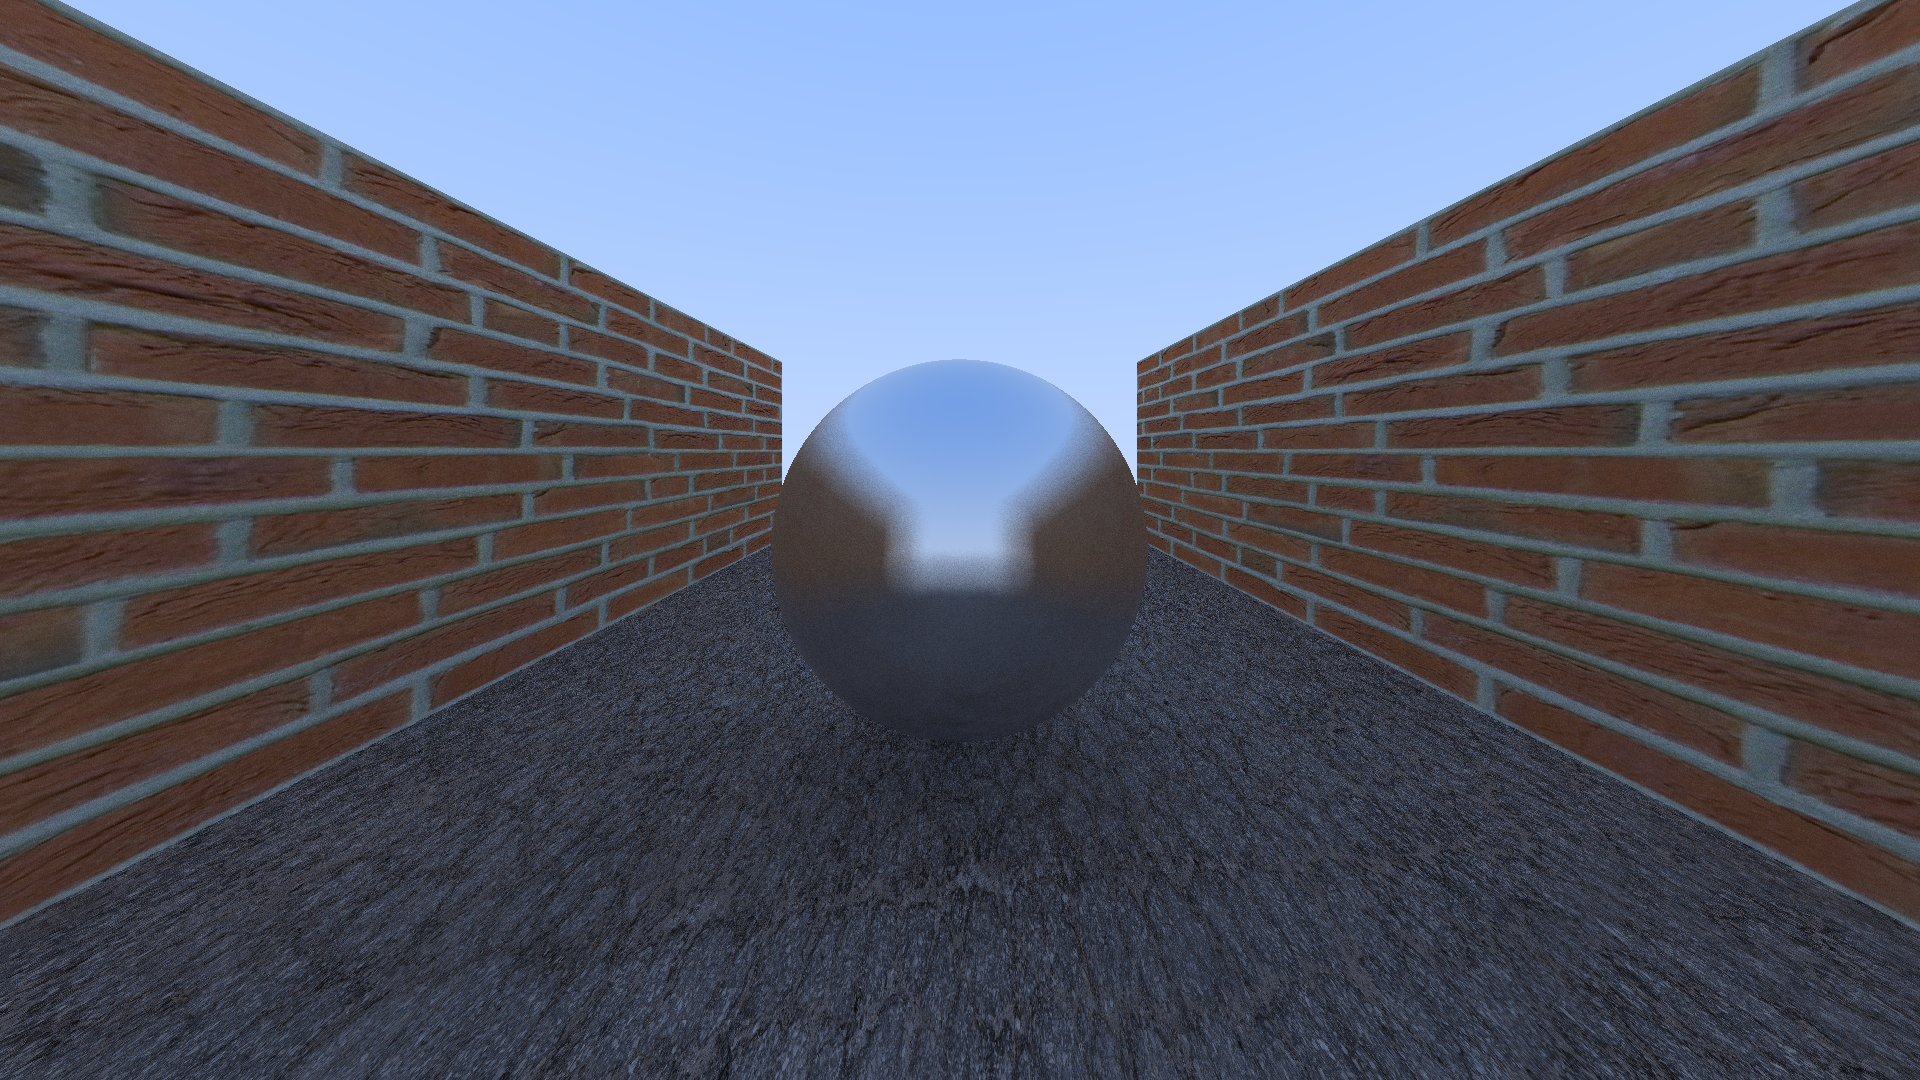
\includegraphics[width=15cm]{../result/result.png}

% \newpage
\subsection*{Выводы}

В ходе выполнения лабораторной работы была реализована сцена с использованием трассировки лучей.
Лучи также учитывали текстуры объектов при отражении. Я изучил основные методы трассировки лучей, а также
определение пересечений лучей с объектами.

\end{document}